\appendix

\section{Syntax Table}\label{sec:Syntax}
\begin{tabular}{ |c|c|c| }
    \hline
    \textbf{Name}        & \textbf{Abstract Syntax}   & \textbf{Concrete Syntax} \\
    \hline
    Empty string         & $\epsilon$                 & $-$                      \\
    \hline
    Match                & $a$                        & $a$                      \\
                         &                            & $<ab>$                   \\
    \hline
    Match any            & $x$                        & $.$                      \\
    \hline
    Order of operations  & $-$                        & $(a)$                    \\
    \hline
    Union                & $\varphi_1\vee\varphi_2$   & $a \mid b$               \\
    \hline
    Intersection         & $\varphi_1\wedge\varphi_2$ & $a\&b$                   \\
    \hline
    Concatenation        & $\varphi_1\cdot\varphi_2$  & $ab$                     \\
    \hline
    Absorbed             &                            &                          \\
    concatenation        & $\varphi_1\circ\varphi_2$  & $a'b$                    \\
    \hline
    Guaranteed iteration & $\varphi^+$                & $a+$                     \\
    \hline
    Absorbed             &                            &                          \\
    guaranteed iteration & $\varphi^\oplus$           & $a+'$                    \\
    \hline
    Iteration            & $\varphi_1*$               & $a*$                     \\
    \hline
    Absorbed iteration   & $\varphi_1\ostar\varphi_2$ & $a*'$                    \\
    \hline
    Interval             & $\varphi_I$                & $a[t_1;t_2]$             \\
                         &                            & $a[t_1;t_2[$             \\
                         &                            & $a]t_1;t_2]$             \\
                         &                            & $a]t_1;t_2[$             \\
    \hline
    Rename               & $\theta(\varphi)$          & $a\{a0,b1\}$             \\
    \hline
\end{tabular}

\newpage
\section{Precedence Table}\label{sec:Precedence}
Precedence of operators ordered, so first row has the highest precedence.

\begin{tabular}{ |c| }
    \hline
    \textbf{Precedence Table} \\
    \hline
    $(a)$ \quad
    $a$ \quad
    $<ab>$ \quad
    $.$                       \\
    \hline
    $a[t_1;t_2]$ \quad
    $a[t_1;t_2[$ \quad
    $a]t_1;t_2]$ \quad
    $a]t_1;t_2[$              \\
    \hline
    $a+$ \quad
    $a+'$ \quad
    $a*$ \quad
    $a*'$                     \\
    \hline
    $ab$ \quad
    $a'b$                     \\
    \hline
    $a|b$                     \\
    \hline
    $a\&b$                    \\
    \hline
    $a\{a0,b1\}$              \\
    \hline
\end{tabular}

\newpage
\section{Correction for paper}\label{sec:PaperCorrections}
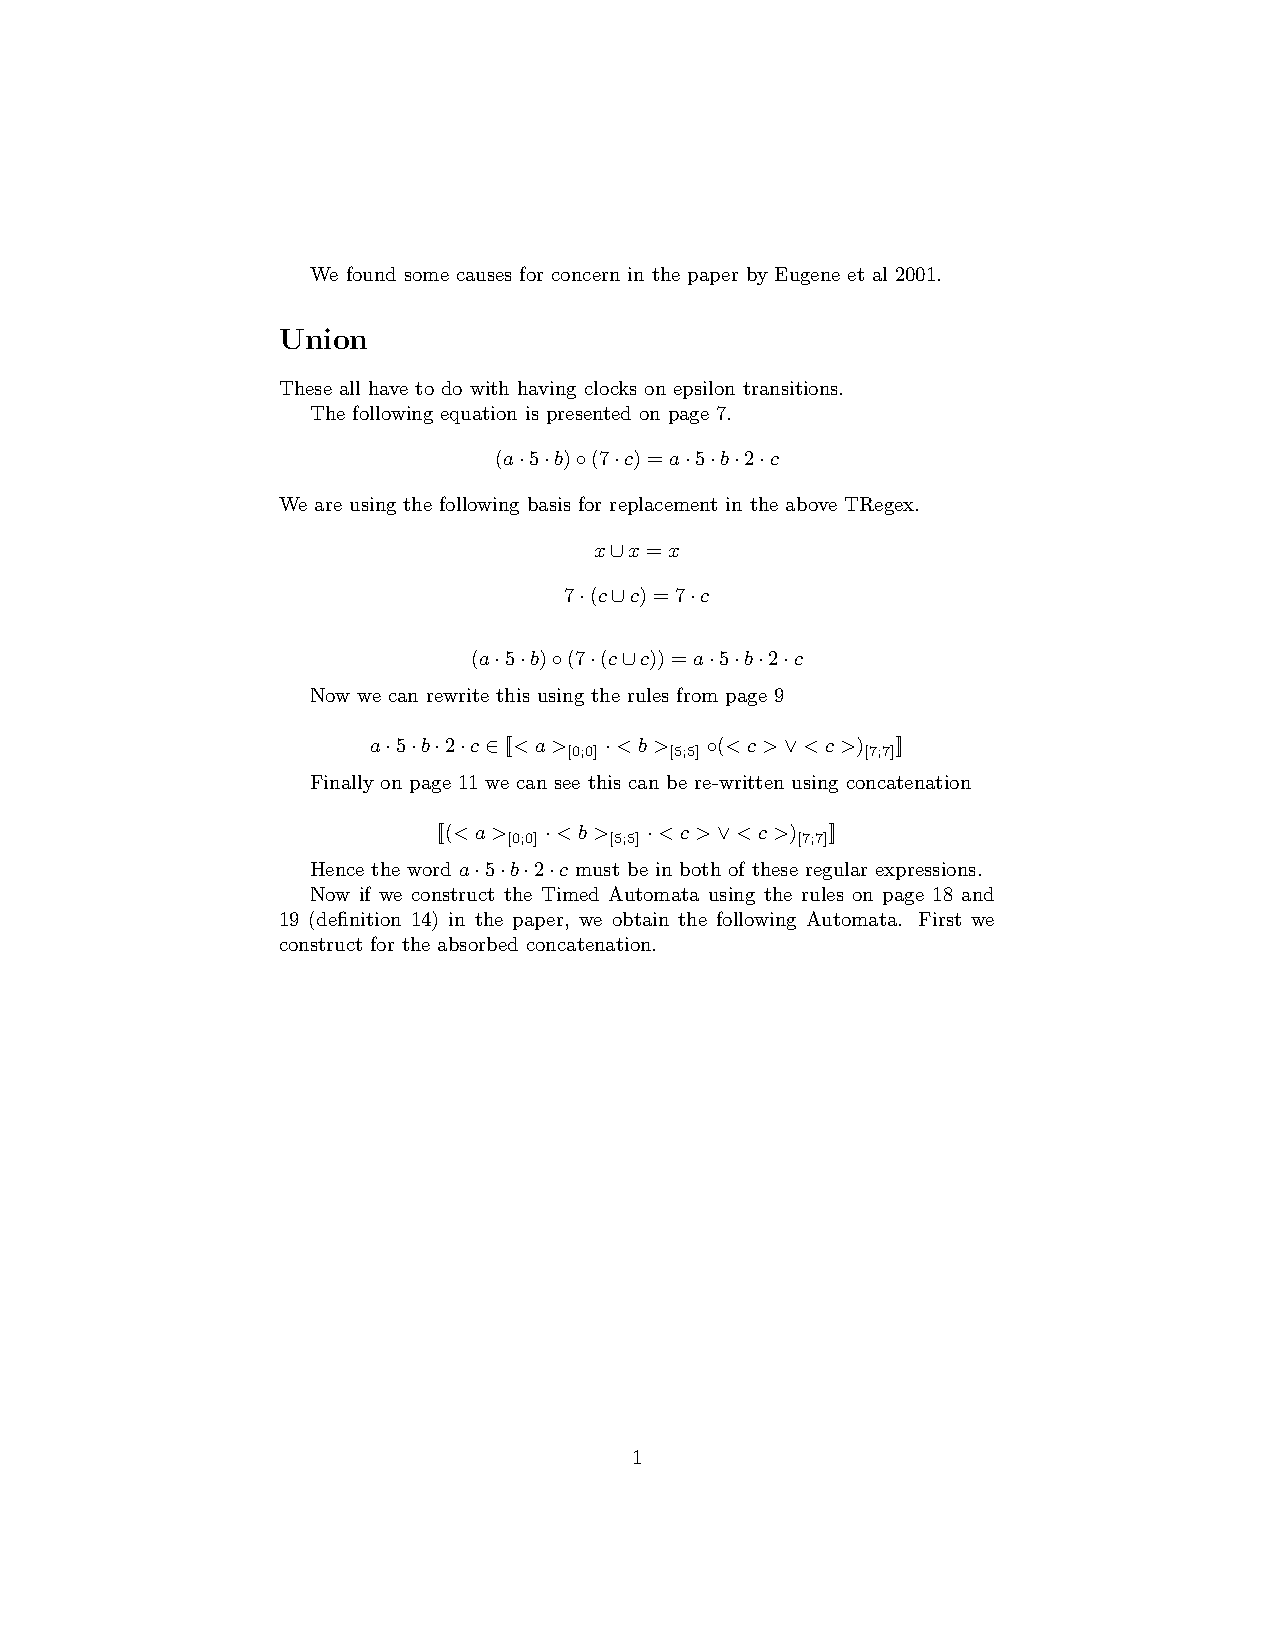
\includepdf[pages=-]{Documents/Appendix/PaperProblems.pdf}

\section{Regular Expressions}\label{sec:RegularExpressions}
\label{app:RegularExpressionTable}
$$p_l=\str{(}$$
$$p_r=\str{)}$$
$$a=\str{+'}$$
$$i=\str{|}$$
$$s=\str{j}$$
$$i_1=\str{j[1;10]}$$
$$i_2=\str{j[1;1]}$$

$$a(n)=p_l^n \circ s \circ (p_r \circ a)^n$$
$$b(n)=p_l^n \circ i_1 \circ (p_r \circ a)^n$$
$$c(n)=i_1^n \circ i \circ i_2$$
$$d(n)=s^n \circ i \circ s$$
$$e(n)=s^n \circ a$$
$$f(n)=(i_2 \circ i)^{n-1} \circ i_2$$

\begin{tabular}{|c|c|}
    \hline
    index & expression \\
    \hline
    0  & a(1) \\
    1  & a(2) \\
    2  & a(4) \\
    \hline
    3  & b(1) \\
    4  & b(2) \\
    5  & b(4) \\
    \hline
    6  & c(64) \\
    7  & c(128) \\
    8  & c(256) \\
    \hline
    9  & d(64) \\
    10 & d(128) \\
    11 & d(256) \\
    \hline
    12 & e(64) \\
    13 & e(128) \\
    14 & e(256) \\
    \hline
    15 & f(1) \\
    16 & f(2) \\
    17 & f(4) \\
    18 & f(8) \\
    19 & f(16) \\
    \hline
\end{tabular}

\newpage
\section{Benchmark table}\label{sec:BenchmarkTable}
BenchmarkDotNet v0.13.12, EndeavourOS
Intel Core i9-9900K CPU 3.60GHz (Coffee Lake), 1 CPU, 16 logical and 8 physical cores
.NET SDK 8.0.104
  [Host]    : .NET 8.0.4 (8.0.424.16909), X64 RyuJIT AVX2
  MediumRun : .NET 8.0.4 (8.0.424.16909), X64 RyuJIT AVX2
Job=MediumRun  Runtime=.NET 8.0  Toolchain=net8.0  
IterationCount=15  LaunchCount=2  WarmupCount=10  

\begin{sidewaystable}
    \begin{tabular}{|c|c|c|c|c|c|c|c|c|c|}
        \hline
        Method  &   regex   &   Mean                  &   Error             &   StdDev                &   Median                &   Gen0        &   Gen1        &   Gen2        &   Allocated        \\
        \hline
        N       &   0       &   1,634.9 ns            &   9.87 ns           &   14.47 ns              &   1,642.0 ns            &   0.0610      &   0.0000      &   0.0000      &   5.04 KB          \\
        E       &   0       &   2,130.0 ns            &   11.54 ns          &   16.55 ns              &   2,136.5 ns            &   0.0725      &   0.0000      &   0.0000      &   5.98 KB          \\
        S       &   0       &   2,027.1 ns            &   6.68 ns           &   9.14 ns               &   2,028.0 ns            &   0.0687      &   0.0000      &   0.0000      &   5.89 KB          \\
        SS      &   0       &   2,348.2 ns            &   4.18 ns           &   5.86 ns               &   2,348.6 ns            &   0.0801      &   0.0000      &   0.0000      &   6.72 KB          \\
        SE      &   0       &   2,417.8 ns            &   12.02 ns          &   17.62 ns              &   2,408.9 ns            &   0.0801      &   0.0000      &   0.0000      &   6.81 KB          \\
        ES      &   0       &   2,394.1 ns            &   7.05 ns           &   10.33 ns              &   2,397.4 ns            &   0.0801      &   0.0000      &   0.0000      &   6.81 KB          \\
        EE      &   0       &   2,461.5 ns            &   12.50 ns          &   16.25 ns              &   2,459.4 ns            &   0.0839      &   0.0000      &   0.0000      &   6.91 KB          \\
        N       &   1       &   6,036.6 ns            &   56.42 ns          &   82.70 ns              &   6,097.2 ns            &   0.1755      &   0.0000      &   0.0000      &   14.63 KB         \\
        E       &   1       &   8,039.4 ns            &   37.01 ns          &   55.40 ns              &   8,033.7 ns            &   0.2136      &   0.0000      &   0.0000      &   17.63 KB         \\
        S       &   1       &   6,962.4 ns            &   143.05 ns         &   200.54 ns             &   6,799.6 ns            &   0.1907      &   0.0000      &   0.0000      &   15.67 KB         \\
        SS      &   1       &   7,674.8 ns            &   186.12 ns         &   278.58 ns             &   7,669.3 ns            &   0.2060      &   0.0000      &   0.0000      &   17.33 KB         \\
        SE      &   1       &   8,672.8 ns            &   43.27 ns          &   64.77 ns              &   8,675.9 ns            &   0.2289      &   0.0000      &   0.0000      &   19.28 KB         \\
        ES      &   1       &   7,637.9 ns            &   13.79 ns          &   20.21 ns              &   7,645.1 ns            &   0.2136      &   0.0000      &   0.0000      &   17.52 KB         \\
        EE      &   1       &   8,800.2 ns            &   22.93 ns          &   33.62 ns              &   8,798.2 ns            &   0.2289      &   0.0000      &   0.0000      &   19.47 KB         \\
        N       &   2       &   365,861.8 ns          &   1,766.60 ns       &   2,644.17 ns           &   365,384.0 ns          &   7.8125      &   1.9531      &   0.0000      &   668.95 KB        \\
        E       &   2       &   530,259.4 ns          &   7,480.44 ns       &   10,964.74 ns          &   521,403.1 ns          &   11.7188     &   2.9297      &   0.0000      &   971.15 KB        \\
        S       &   2       &   394,797.3 ns          &   576.68 ns          &   863.15 ns             &   394,564.5 ns          &   8.3008      &   2.4414      &   0.0000      &   679.97 KB        \\
        SS      &   2       &   402,027.0 ns          &   936.47 ns          &   1,343.05 ns           &   402,349.1 ns          &   8.3008      &   2.4414      &   0.0000      &   684.61 KB        \\
        SE      &   2       &   533,352.9 ns          &   1,004.86 ns       &   1,472.92 ns           &   533,494.6 ns          &   11.7188     &   2.9297      &   0.0000      &   975.79 KB        \\
        ES      &   2       &   270,858.2 ns          &   1,131.18 ns       &   1,693.10 ns           &   271,188.1 ns          &   6.8359      &   1.4648      &   0.0000      &   566.77 KB        \\
        EE      &   2       &   368,669.7 ns          &   1,670.77 ns       &   2,500.73 ns           &   367,754.5 ns          &   9.2773      &   1.9531      &   0.0000      &   768.92 KB        \\
        N       &   3       &   5,352.0 ns            &   133.94 ns          &   196.33 ns             &   5,504.3 ns            &   0.1526      &   0.0000      &   0.0000      &   12.73 KB         \\
        E       &   3       &   7,892.0 ns            &   40.73 ns           &   55.75 ns              &   7,911.1 ns            &   0.1984      &   0.0000      &   0.0000      &   16.92 KB         \\
        S       &   3       &   6,849.0 ns            &   14.18 ns           &   19.88 ns              &   6,843.2 ns            &   0.1831      &   0.0000      &   0.0000      &   15.16 KB         \\
        SS      &   3       &   5,774.6 ns            &   52.84 ns           &   75.78 ns              &   5,754.8 ns            &   0.1602      &   0.0000      &   0.0000      &   13.2 KB          \\
        SE      &   3       &   6,492.7 ns            &   14.03 ns           &   21.00 ns              &   6,493.8 ns            &   0.1755      &   0.0000      &   0.0000      &   14.71 KB         \\
        ES      &   3       &   6,098.4 ns            &   8.54 ns            &   11.98 ns              &   6,093.4 ns            &   0.1678      &   0.0000      &   0.0000      &   14.21 KB         \\
        EE      &   3       &   6,843.2 ns            &   14.32 ns           &   21.43 ns              &   6,850.9 ns            &   0.1907      &   0.0000      &   0.0000      &   15.73 KB         \\
        N       &   4       &   33,275.6 ns           &   252.37 ns         &   361.95 ns             &   33,037.8 ns           &   0.8545      &   0.0000      &   0.0000      &   69.88 KB         \\
        E       &   4       &   46,225.8 ns           &   59.53 ns          &   89.10 ns              &   46,228.2 ns           &   1.0986      &   0.0610      &   0.0000      &   89.88 KB         \\
        S       &   4       &   39,386.9 ns           &   129.39 ns         &   189.65 ns             &   39,293.8 ns           &   0.9155      &   0.0000      &   0.0000      &   76.1 KB          \\
        SS      &   4       &   18,779.8 ns           &   40.31 ns          &   56.51 ns              &   18,777.7 ns           &   0.4578      &   0.0000      &   0.0000      &   38.41 KB         \\
        SE      &   4       &   21,796.9 ns           &   91.81 ns          &   131.67 ns             &   21,810.0 ns           &   0.5188      &   0.0000      &   0.0000      &   44.69 KB         \\
        ES      &   4       &   17,999.6 ns           &   154.18 ns         &   221.13 ns             &   18,123.7 ns           &   0.4578      &   0.0000      &   0.0000      &   38.64 KB         \\
        EE      &   4       &   20,351.3 ns           &   190.70 ns         &   267.34 ns             &   20,166.2 ns           &   0.5188      &   0.0000      &   0.0000      &   42.84 KB         \\
        N       &   5       &   14,345,441.6 ns       &   106,317.27 ns     &   155,838.48 ns         &   14,360,473.9 ns       &   234.3750    &   218.7500    &   109.3750    &   16675.07 KB      \\
        E       &   5       &   21,889,111.1 ns       &   263,640.17 ns     &   369,586.70 ns         &   21,986,565.8 ns       &   343.7500    &   312.5000    &   125.0000    &   26493.89 KB      \\
        S       &   5       &   15,581,794.2 ns       &   57,071.73 ns      &   85,422.28 ns          &   15,575,622.0 ns       &   234.3750    &   218.7500    &   109.3750    &   17172.08 KB      \\
        SS      &   5       &   6,445,558.3 ns        &   68,269.20 ns      &   102,182.12 ns         &   6,426,665.7 ns        &   93.7500     &   78.1250     &   31.2500     &   7064.14 KB       \\
        SE      &   5       &   9,163,154.7 ns        &   77,369.76 ns      &   115,803.41 ns         &   9,179,374.2 ns        &   140.6250    &   125.0000    &   46.8750     &   11009.93 KB      \\
        ES      &   5       &   3,569,375.9 ns        &   10,572.83 ns      &   15,163.23 ns          &   3,574,975.3 ns        &   58.5938     &   54.6875     &   27.3438     &   4924.5 KB        \\
        EE      &   5       &   5,761,799.7 ns        &   18,151.44 ns      &   24,231.65 ns          &   5,756,398.0 ns        &   101.5625    &   93.7500     &   31.2500     &   7486.67 KB       \\
        \hline
    \end{tabular}
\end{sidewaystable}
\begin{sidewaystable}
    \begin{tabular}{|c|c|c|c|c|c|c|c|c|c|}
        \hline
        Method  &   regex   &   Mean                  &   Error             &   StdDev                &   Median                &   Gen0        &   Gen1        &   Gen2        &   Allocated        \\
        \hline
        N       &   6       &   1,058,482.1 ns        &   4,507.33 ns       &   6,318.65 ns           &   1,055,488.1 ns        &   33.2031     &   13.6719     &   0.0000      &   2774.94 KB       \\
        E       &   6       &   130,202,842.2 ns      &   1,165,246.45 ns   &   1,744,086.02 ns       &   130,263,725.1 ns      &   1750.0000   &   500.0000    &   0.0000      &   158752.09 KB     \\
        S       &   6       &   1,087,341.0 ns        &   4,657.28 ns       &   6,679.32 ns           &   1,086,714.2 ns        &   33.2031     &   13.6719     &   0.0000      &   2799.35 KB       \\
        SS      &   6       &   882,452.6 ns          &   13,988.79 ns      &   19,610.32 ns          &   866,000.2 ns          &   28.3203     &   12.6953     &   0.0000      &   2338.61 KB       \\
        SE      &   6       &   40,407,196.0 ns       &   71,260.18 ns      &   104,452.24 ns         &   40,386,796.0 ns       &   153.8462    &   0.0000      &   0.0000      &   14810.97 KB      \\
        ES      &   6       &   176,619,156.3 ns      &   289,428.88 ns     &   415,090.25 ns         &   176,570,478.8 ns      &   1333.3333   &   333.3333    &   0.0000      &   112051.15 KB     \\
        EE      &   6       &   218,959,171.3 ns      &   546,414.44 ns     &   783,651.26 ns         &   219,103,037.2 ns      &   1333.3333   &   333.3333    &   0.0000      &   124523.45 KB     \\
        N       &   7       &   3,484,513.8 ns        &   29,916.06 ns      &   44,776.95 ns          &   3,486,315.8 ns        &   117.1875    &   113.2813    &   0.0000      &   9617.03 KB       \\
        E       &   7       &   1,547,147,583.4 ns    &   8,026,410.82 ns   &   11,765,008.91 ns      &   1,549,048,615.0 ns    &   15000.0000  &   1000.0000   &   0.0000      &   1245220.51 KB    \\
        S       &   7       &   3,566,171.7 ns        &   13,619.88 ns      &   19,963.84 ns          &   3,574,351.7 ns        &   117.1875    &   89.8438     &   0.0000      &   9667.24 KB       \\
        SS      &   7       &   3,037,890.7 ns        &   4,994.25 ns       &   7,475.16 ns           &   3,036,768.7 ns        &   105.4688    &   82.0313     &   0.0000      &   8618.71 KB       \\
        SE      &   7       &   548,214,611.6 ns      &   3,979,121.03 ns   &   5,955,761.00 ns       &   548,884,287.0 ns      &   1000.0000   &   0.0000      &   0.0000      &   102171.73 KB     \\
        ES      &   7       &   2,454,885,536.6 ns    &   4,488,862.38 ns   &   6,579,716.27 ns       &   2,454,092,008.0 ns    &   10000.0000  &   1000.0000   &   0.0000      &   884427.52 KB     \\
        EE      &   7       &   2,995,173,650.1 ns    &   18,242,043.28 ns  &   25,572,796.96 ns      &   3,012,707,120.0 ns    &   11000.0000  &   1000.0000   &   0.0000      &   977979.83 KB     \\
        N       &   8       &   12,697,373.2 ns       &   21,288.66 ns      &   29,843.72 ns          &   12,697,516.0 ns       &   437.5000    &   421.8750    &   0.0000      &   36055.38 KB      \\
        E       &   8       &   21,617,377,726.5 ns   &   288,524,813.91 ns &   431,850,356.17 ns     &   21,785,903,112.0 ns   &   120000.0000 &   3000.0000   &   1000.0000   &   9871874.21 KB    \\
        S       &   8       &   12,737,119.2 ns       &   118,281.48 ns     &   177,038.15 ns         &   12,737,861.9 ns       &   437.5000    &   421.8750    &   0.0000      &   36160.29 KB      \\
        SS      &   8       &   11,038,197.9 ns       &   124,283.70 ns     &   178,243.96 ns         &   11,168,117.2 ns       &   390.6250    &   375.0000    &   0.0000      &   33125.43 KB      \\
        SE      &   8       &   8,368,043,360.9 ns    &   48,410,361.58 ns  &   72,458,349.80 ns      &   8,392,358,432.5 ns    &   9000.0000   &   1000.0000   &   0.0000      &   756806.44 KB     \\
        ES      &   8       &   34,743,709,646.1 ns   &   671,871,810.11 ns &   963,578,473.62 ns     &   33,914,698,636.5 ns   &   86000.0000  &   4000.0000   &   1000.0000   &   7031719.82 KB    \\
        EE      &   8       &   42,989,588,867.6 ns   &   984,507,838.03 ns &   1,473,564,976.07 ns   &   42,965,379,610.5 ns   &   94000.0000  &   5000.0000   &   1000.0000   &   7755400.13 KB    \\
        N       &   9       &   466,234.1 ns          &   3,325.83 ns       &   4,977.94 ns           &   466,314.1 ns          &   17.0898     &   3.9063      &   0.0000      &   1433.59 KB       \\
        E       &   9       &   498,700.1 ns          &   2,530.69 ns       &   3,547.67 ns           &   496,592.0 ns          &   17.5781     &   3.9063      &   0.0000      &   1450.21 KB       \\
        S       &   9       &   495,040.8 ns          &   1,200.99 ns       &   1,797.58 ns           &   494,859.9 ns          &   17.5781     &   2.9297      &   0.0000      &   1449.53 KB       \\
        SS      &   9       &   480,547.2 ns          &   2,326.44 ns       &   3,482.11 ns           &   480,458.0 ns          &   17.0898     &   3.4180      &   0.0000      &   1412.54 KB       \\
        SE      &   9       &   479,276.2 ns          &   2,269.46 ns       &   3,326.54 ns           &   477,245.7 ns          &   17.0898     &   3.4180      &   0.0000      &   1413.22 KB       \\
        ES      &   9       &   488,593.6 ns          &   1,034.18 ns       &   1,483.18 ns           &   488,766.5 ns          &   16.6016     &   3.9063      &   0.0000      &   1419.92 KB       \\
        EE      &   9       &   485,500.6 ns          &   1,923.13 ns       &   2,818.90 ns           &   486,744.9 ns          &   17.0898     &   3.4180      &   0.0000      &   1420.59 KB       \\
        N       &   10      &   1,552,189.8 ns        &   4,112.69 ns       &   6,155.67 ns           &   1,552,457.7 ns        &   58.5938     &   21.4844     &   0.0000      &   4915.88 KB       \\
        E       &   10      &   1,640,849.7 ns        &   8,326.43 ns       &   12,204.78 ns          &   1,648,903.8 ns        &   60.5469     &   19.5313     &   0.0000      &   4948.77 KB       \\
        S       &   10      &   1,614,288.9 ns        &   11,917.71 ns      &   17,468.83 ns          &   1,622,644.2 ns        &   60.5469     &   13.6719     &   0.0000      &   4948.09 KB       \\
        SS      &   10      &   1,572,649.2 ns        &   10,392.10 ns      &   15,554.41 ns          &   1,572,842.8 ns        &   58.5938     &   19.5313     &   0.0000      &   4872.73 KB       \\
        SE      &   10      &   1,567,464.8 ns        &   2,522.52 ns       &   3,697.48 ns           &   1,567,685.0 ns        &   58.5938     &   21.4844     &   0.0000      &   4873.41 KB       \\
        ES      &   10      &   1,613,948.4 ns        &   3,672.80 ns       &   5,497.28 ns           &   1,612,299.2 ns        &   58.5938     &   17.5781     &   0.0000      &   4887.9 KB        \\
        EE      &   10      &   1,609,730.6 ns        &   9,676.92 ns       &   13,878.34 ns          &   1,608,487.3 ns        &   58.5938     &   19.5313     &   0.0000      &   4888.58 KB       \\
        N       &   11      &   5,441,492.3 ns        &   28,112.35 ns      &   42,077.25 ns          &   5,443,850.1 ns        &   210.9375    &   125.0000    &   0.0000      &   17662.75 KB      \\
        E       &   11      &   5,715,852.7 ns        &   6,080.15 ns       &   8,523.52 ns           &   5,714,072.2 ns        &   210.9375    &   117.1875    &   0.0000      &   17730.58 KB      \\
        S       &   11      &   5,623,561.5 ns        &   15,302.34 ns      &   22,429.97 ns          &   5,620,045.6 ns        &   210.9375    &   117.1875    &   0.0000      &   17729.9 KB       \\
        SS      &   11      &   5,609,644.0 ns        &   11,036.86 ns      &   15,472.14 ns          &   5,608,025.8 ns        &   210.9375    &   109.3750    &   0.0000      &   17579.53 KB      \\
        SE      &   11      &   5,491,159.6 ns        &   23,273.37 ns      &   34,113.80 ns          &   5,488,853.9 ns        &   210.9375    &   125.0000    &   0.0000      &   17580.21 KB      \\
        ES      &   11      &   5,510,257.2 ns        &   10,030.97 ns      &   14,703.27 ns          &   5,509,956.2 ns        &   210.9375    &   101.5625    &   0.0000      &   17611.64 KB      \\
        EE      &   11      &   5,583,399.1 ns        &   38,305.29 ns      &   56,147.39 ns          &   5,545,160.0 ns        &   210.9375    &   109.3750    &   0.0000      &   17612.32 KB      \\
        \hline
    \end{tabular}
\end{sidewaystable}
\begin{sidewaystable}
    \begin{tabular}{|c|c|c|c|c|c|c|c|c|c|}
        \hline
        Method  &   regex   &   Mean                  &   Error             &   StdDev                &   Median                &   Gen0        &   Gen1        &   Gen2        &   Allocated        \\
        \hline
        N       &   12      &   438,380.5 ns          &   1,855.76 ns       &   2,661.48 ns           &   439,950.3 ns          &   16.1133     &   3.4180      &   0.0000      &   1344.23 KB       \\
        E       &   12      &   455,207.0 ns          &   2,573.48 ns       &   3,851.86 ns           &   455,383.9 ns          &   16.6016     &   3.9063      &   0.0000      &   1365.41 KB       \\
        S       &   12      &   454,085.5 ns          &   1,587.65 ns       &   2,225.66 ns           &   452,693.8 ns          &   16.6016     &   3.9063      &   0.0000      &   1358.13 KB       \\
        SS      &   12      &   446,637.5 ns          &   2,502.28 ns       &   3,507.85 ns           &   448,952.7 ns          &   16.6016     &   3.9063      &   0.0000      &   1358.96 KB       \\
        SE      &   12      &   459,558.8 ns          &   3,345.14 ns       &   4,797.50 ns           &   460,456.6 ns          &   16.6016     &   3.9063      &   0.0000      &   1366.24 KB       \\
        ES      &   12      &   450,664.2 ns          &   4,110.95 ns       &   5,762.97 ns           &   453,953.1 ns          &   16.6016     &   3.4180      &   0.0000      &   1359.05 KB       \\
        EE      &   12      &   458,164.2 ns          &   1,655.20 ns       &   2,426.17 ns           &   459,618.3 ns          &   16.6016     &   3.4180      &   0.0000      &   1366.34 KB       \\
        N       &   13      &   1,477,177.5 ns        &   1,462.66 ns       &   2,050.45 ns           &   1,477,241.6 ns        &   56.6406     &   23.4375     &   0.0000      &   4732.96 KB       \\
        E       &   13      &   1,511,804.0 ns        &   6,297.65 ns       &   8,828.43 ns           &   1,510,737.8 ns        &   56.6406     &   23.4375     &   0.0000      &   4777.54 KB       \\
        S       &   13      &   1,501,376.8 ns        &   2,245.42 ns       &   3,291.30 ns           &   1,501,064.8 ns        &   56.6406     &   25.3906     &   0.0000      &   4762.46 KB       \\
        SS      &   13      &   1,530,411.6 ns        &   7,332.51 ns       &   10,516.06 ns          &   1,529,417.4 ns        &   56.6406     &   23.4375     &   0.0000      &   4763.29 KB       \\
        SE      &   13      &   1,525,024.1 ns        &   1,776.38 ns       &   2,547.63 ns           &   1,525,165.1 ns        &   56.6406     &   23.4375     &   0.0000      &   4778.37 KB       \\
        ES      &   13      &   1,521,473.5 ns        &   2,837.26 ns       &   4,158.81 ns           &   1,522,342.5 ns        &   56.6406     &   25.3906     &   0.0000      &   4763.38 KB       \\
        EE      &   13      &   1,532,103.4 ns        &   5,675.10 ns       &   7,955.70 ns           &   1,536,225.3 ns        &   56.6406     &   23.4375     &   0.0000      &   4778.46 KB       \\
        N       &   14      &   5,328,251.7 ns        &   9,635.87 ns       &   13,508.14 ns          &   5,329,462.9 ns        &   210.9375    &   140.6250    &   0.0000      &   17289.26 KB      \\
        E       &   14      &   5,406,084.6 ns        &   19,226.40 ns      &   27,573.93 ns          &   5,406,630.6 ns        &   210.9375    &   140.6250    &   0.0000      &   17384.65 KB      \\
        S       &   14      &   5,323,808.2 ns        &   44,007.39 ns      &   64,505.45 ns          &   5,367,876.2 ns        &   210.9375    &   140.6250    &   0.0000      &   17352.64 KB      \\
        SS      &   14      &   5,503,721.2 ns        &   6,996.40 ns       &   10,034.03 ns          &   5,504,045.1 ns        &   210.9375    &   132.8125    &   0.0000      &   17353.47 KB      \\
        SE      &   14      &   5,348,640.0 ns        &   43,266.43 ns      &   62,051.42 ns          &   5,388,433.8 ns        &   210.9375    &   132.8125    &   0.0000      &   17385.48 KB      \\
        ES      &   14      &   5,359,476.8 ns        &   18,235.38 ns      &   24,960.80 ns          &   5,371,932.9 ns        &   210.9375    &   117.1875    &   0.0000      &   17353.56 KB      \\
        EE      &   14      &   5,515,236.7 ns        &   13,930.15 ns      &   20,418.63 ns          &   5,513,582.8 ns        &   210.9375    &   125.0000    &   0.0000      &   17385.58 KB      \\
        N       &   15      &   625.1 ns              &   2.92 ns           &   4.09 ns               &   624.9 ns              &   0.0286      &   0.0000      &   0.0000      &   2.38 KB          \\
        E       &   15      &   1,512.2 ns            &   3.56 ns           &   5.33 ns               &   1,511.6 ns            &   0.0572      &   0.0000      &   0.0000      &   4.75 KB          \\
        S       &   15      &   1,117.2 ns            &   3.44 ns           &   5.04 ns               &   1,117.0 ns            &   0.0439      &   0.0000      &   0.0000      &   3.73 KB          \\
        SS      &   15      &   1,125.3 ns            &   5.79 ns           &   8.66 ns               &   1,128.6 ns            &   0.0439      &   0.0000      &   0.0000      &   3.73 KB          \\
        SE      &   15      &   1,511.3 ns            &   2.95 ns           &   4.41 ns               &   1,511.1 ns            &   0.0572      &   0.0000      &   0.0000      &   4.75 KB          \\
        ES      &   15      &   1,130.7 ns            &   2.07 ns           &   3.09 ns               &   1,130.8 ns            &   0.0439      &   0.0000      &   0.0000      &   3.73 KB          \\
        EE      &   15      &   1,507.7 ns            &   3.85 ns           &   5.76 ns               &   1,507.3 ns            &   0.0572      &   0.0000      &   0.0000      &   4.75 KB          \\
        N       &   16      &   4,363.0 ns            &   7.50 ns           &   11.00 ns              &   4,362.4 ns            &   0.1450      &   0.0000      &   0.0000      &   12.3 KB          \\
        E       &   16      &   6,262.7 ns            &   11.33 ns          &   16.25 ns              &   6,264.8 ns            &   0.1831      &   0.0000      &   0.0000      &   15.5 KB          \\
        S       &   16      &   5,341.5 ns            &   12.86 ns          &   18.03 ns              &   5,339.1 ns            &   0.1678      &   0.0000      &   0.0000      &   13.86 KB         \\
        SS      &   16      &   4,758.7 ns            &   42.89 ns          &   64.20 ns              &   4,750.0 ns            &   0.1602      &   0.0000      &   0.0000      &   13.37 KB         \\
        SE      &   16      &   5,500.0 ns            &   35.59 ns          &   53.27 ns              &   5,500.8 ns            &   0.1755      &   0.0000      &   0.0000      &   14.63 KB         \\
        ES      &   16      &   5,522.4 ns            &   43.80 ns          &   62.82 ns              &   5,477.6 ns            &   0.1831      &   0.0000      &   0.0000      &   15.4 KB          \\
        EE      &   16      &   6,226.0 ns            &   83.36 ns          &   122.19 ns             &   6,319.5 ns            &   0.1984      &   0.0000      &   0.0000      &   16.66 KB         \\
        N       &   17      &   23,745.2 ns           &   49.79 ns          &   74.52 ns              &   23,749.4 ns           &   0.7019      &   0.0305      &   0.0000      &   59.38 KB         \\
        E       &   17      &   34,755.7 ns           &   254.33 ns         &   364.76 ns             &   34,751.1 ns           &   0.9766      &   0.0000      &   0.0000      &   83.24 KB         \\
        S       &   17      &   26,400.8 ns           &   37.83 ns          &   55.46 ns              &   26,394.5 ns           &   0.7324      &   0.0305      &   0.0000      &   62.1 KB          \\
        SS      &   17      &   12,385.5 ns           &   80.16 ns          &   117.49 ns             &   12,404.3 ns           &   0.3967      &   0.0000      &   0.0000      &   33.36 KB         \\
        SE      &   17      &   13,643.0 ns           &   72.74 ns          &   108.87 ns             &   13,646.4 ns           &   0.4272      &   0.0000      &   0.0000      &   36.13 KB         \\
        ES      &   17      &   15,279.1 ns           &   166.63 ns         &   238.98 ns             &   15,109.0 ns           &   0.4578      &   0.0000      &   0.0000      &   39.59 KB         \\
        EE      &   17      &   15,860.8 ns           &   102.35 ns         &   146.79 ns             &   15,930.8 ns           &   0.4883      &   0.0000      &   0.0000      &   40.86 KB         \\
        \hline
    \end{tabular}
\end{sidewaystable}
\begin{sidewaystable}
    \begin{tabular}{|c|c|c|c|c|c|c|c|c|c|}
        \hline
        Method  &   regex   &   Mean                  &   Error             &   StdDev                &   Median                &   Gen0        &   Gen1        &   Gen2        &   Allocated        \\
        \hline
        N       &   18      &   404,847.5 ns          &   2,978.33 ns       &   4,457.83 ns           &   404,539.6 ns          &   11.2305     &   1.9531      &   0.0000      &   917.55 KB        \\
        E       &   18      &   1,039,886.9 ns        &   2,864.49 ns       &   4,198.73 ns           &   1,041,291.5 ns        &   29.2969     &   13.6719     &   0.0000      &   2515.32 KB       \\
        S       &   18      &   441,169.9 ns          &   1,979.55 ns       &   2,839.01 ns           &   442,855.6 ns          &   11.2305     &   4.3945      &   0.0000      &   934.43 KB        \\
        SS      &   18      &   29,107.9 ns           &   100.08 ns         &   146.70 ns             &   29,081.2 ns           &   0.9155      &   0.0305      &   0.0000      &   76.75 KB         \\
        SE      &   18      &   33,642.9 ns           &   89.41 ns          &   128.23 ns             &   33,611.3 ns           &   1.0376      &   0.0000      &   0.0000      &   86.02 KB         \\
        ES      &   18      &   35,954.9 ns           &   194.75 ns         &  279.30 ns              &   35,966.1 ns           &   1.0376      &   0.0000      &   0.0000      &   89.39 KB         \\
        EE      &   18      &   36,579.7 ns           &   63.92 ns          &   93.69 ns              &   36,585.2 ns           &   1.0986      &   0.0000      &   0.0000      &   90.66 KB         \\
        N       &   19      &   388,956,329.8 ns      &   25,239,927.44 ns  &   37,777,934.96 ns      &   396,098,198.0 ns      &   6000.0000   &   6000.0000   &   4000.0000   &   315469.2 KB      \\
        E       &   19      &   2,007,281,088.0 ns    &   63,324,812.08 ns  &   90,818,553.26 ns      &   2,036,489,152.5 ns    &   27000.0000  &   9000.0000   &   5000.0000   &   1955655.8 KB     \\
        S       &   19      &   439,493,172.0 ns      &   25,717,693.35 ns  &   36,883,547.32 ns      &   449,660,552.0 ns      &   6000.0000   &   6000.0000   &   4000.0000   &   321366.52 KB     \\
        SS      &   19      &   69,831.3 ns           &   180.95 ns           &   270.84 ns             &   69,889.2 ns           &   2.0752      &   0.1221      &   0.0000      &   174.71 KB        \\
        SE      &   19      &   85,871.9 ns           &   412.77 ns           &   591.99 ns             &   85,651.6 ns           &   2.4414      &   0.1221      &   0.0000      &   208.98 KB        \\
        ES      &   19      &   85,025.0 ns           &   159.55 ns           &   233.87 ns             &   85,044.3 ns           &   2.3193      &   0.1221      &   0.0000      &   193.98 KB        \\
        EE      &   19      &   87,248.7 ns           &   784.32 ns           &   1,149.64 ns           &   87,974.0 ns           &   2.3193      &   0.1221      &   0.0000      &   195.24 KB        \\
        \hline    
    \end{tabular}
\end{sidewaystable}

\newpage
\section{Benchmark graphs}\label{sec:BenchmarkGraphs}
\subsection{0-2}
\resizebox{\textwidth}{!}{
    % 0,1,2
\plot{1,2,4}
{(1,1634.9)(2,6036.6)(4,365861.8)}
{(1,2130.0)(2,8039.4)(4,530259.4)}
{(1,2027.1)(2,6962.4)(4,394797.3)}
{(1,2348.2)(2,7674.8)(4,402027)}
{(1,2417.8)(2,8672.8)(4,533352.9)}
{(1,2394.1)(2,7637.9)(4,270858.2)}
{(1,2461.5)(2,8800.2)(4,368669.7)}
    % 0,1,2
\plot{1,2,4}
{(1,1634.9)(2,6036.6)(4,365861.8)}
{(1,2130.0)(2,8039.4)(4,530259.4)}
{(1,2027.1)(2,6962.4)(4,394797.3)}
{(1,2348.2)(2,7674.8)(4,402027)}
{(1,2417.8)(2,8672.8)(4,533352.9)}
{(1,2394.1)(2,7637.9)(4,270858.2)}
{(1,2461.5)(2,8800.2)(4,368669.7)}
}
\subsection{3-5}
\resizebox{\textwidth}{!}{
    % 3,4,5
\plot{1,2,4}
{(1,5352.0)(2,33275.6)(4,14345441.6)}
{(1,7892.0)(2,46225.8)(4,21889111.1)}
{(1,6849.0)(2,39386.9)(4,15581794.2)}
{(1,5774.6)(2,18779.8)(4,6445558.3)}
{(1,6492.7)(2,21796.9)(4,9163154.7)}
{(1,6098.4)(2,17999.6)(4,3569375.9)}
{(1,6843.2)(2,20351.3)(4,5761799.7)}
    % 3,4,5
\plot{1,2,4}
{(1,5352.0)(2,33275.6)(4,14345441.6)}
{(1,7892.0)(2,46225.8)(4,21889111.1)}
{(1,6849.0)(2,39386.9)(4,15581794.2)}
{(1,5774.6)(2,18779.8)(4,6445558.3)}
{(1,6492.7)(2,21796.9)(4,9163154.7)}
{(1,6098.4)(2,17999.6)(4,3569375.9)}
{(1,6843.2)(2,20351.3)(4,5761799.7)}
}
\subsection{6-8}
\resizebox{\textwidth}{!}{
    % 6,7,8
\plotmem{64,128,256}
{(64,2774.94)    (128,9617.03)     (256,36055.38)}
{(64,158752.09)  (128,1245220.51)  (256,9871874.21)}
{(64,2799.35)    (128,9667.24)     (256,36160.29)}
{(64,2338.61)    (128,8618.71)     (256,33125.43)}
{(64,14810.97)   (128,102171.73)  (256,756806.44)}
{(64,112051.15)  (128,884427.52)  (256,7031719.82)}
{(64,124523.45)  (128,977979.83)  (256,7755400.13)}
    % 6,7,8
\plotmem{64,128,256}
{(64,2774.94)    (128,9617.03)     (256,36055.38)}
{(64,158752.09)  (128,1245220.51)  (256,9871874.21)}
{(64,2799.35)    (128,9667.24)     (256,36160.29)}
{(64,2338.61)    (128,8618.71)     (256,33125.43)}
{(64,14810.97)   (128,102171.73)  (256,756806.44)}
{(64,112051.15)  (128,884427.52)  (256,7031719.82)}
{(64,124523.45)  (128,977979.83)  (256,7755400.13)}
}
\subsection{9-11}
\resizebox{\textwidth}{!}{
    % 9,10,11
\plotmem{64,128,256}
{(64,1433.59)(128,4915.88)(256,17662.75)}
{(64,1450.21)(128,4948.77)(256,17730.58)}
{(64,1449.53)(128,4948.09)(256,17729.9)}
{(64,1412.54)(128,4872.73)(256,17579.53)}
{(64,1413.22)(128,4873.41)(256,17580.21)}
{(64,1419.92)(128,4887.9)(256,17611.64)}
{(64,1420.59)(128,4888.58)(256,17612.32)}
    % 9,10,11
\plotmem{64,128,256}
{(64,1433.59)(128,4915.88)(256,17662.75)}
{(64,1450.21)(128,4948.77)(256,17730.58)}
{(64,1449.53)(128,4948.09)(256,17729.9)}
{(64,1412.54)(128,4872.73)(256,17579.53)}
{(64,1413.22)(128,4873.41)(256,17580.21)}
{(64,1419.92)(128,4887.9)(256,17611.64)}
{(64,1420.59)(128,4888.58)(256,17612.32)}
}
\subsection{12-14}
\resizebox{\textwidth}{!}{
    % 12,13,14
\plotmem{64,128,256}
{(64,1344.23)(128,4732.96)(256,17289.26)}
{(64,1365.41)(128,4777.54)(256,17384.65)}
{(64,1358.13)(128,4762.46)(256,17352.64)}
{(64,1358.96)(128,4763.29)(256,17353.47)}
{(64,1366.24)(128,4778.37)(256,17385.48)}
{(64,1359.05)(128,4763.38)(256,17353.56)}
{(64,1366.34)(128,4778.46)(256,17385.58)}
    % 12,13,14
\plotmem{64,128,256}
{(64,1344.23)(128,4732.96)(256,17289.26)}
{(64,1365.41)(128,4777.54)(256,17384.65)}
{(64,1358.13)(128,4762.46)(256,17352.64)}
{(64,1358.96)(128,4763.29)(256,17353.47)}
{(64,1366.24)(128,4778.37)(256,17385.48)}
{(64,1359.05)(128,4763.38)(256,17353.56)}
{(64,1366.34)(128,4778.46)(256,17385.58)}
}
\subsection{15-19}
\resizebox{\textwidth}{!}{
    % 15,16,17,18,19
\plotmem{1,2,4,8,16}
{(1,2.38) (2,12.3)(4,59.38)(8,917.55)   (16,315469.2)}
{(1,4.75)(2,15.5)(4,83.24)(8,2515.32)  (16,1955655.8)}
{(1,3.73)(2,13.86)(4,62.1)(8,934.43)   (16,321366.52)}
{(1,3.73)(2,13.37)(4,33.36)(8,76.75)    (16,174.71)}
{(1,4.75)(2,14.63)(4,36.13)(8,86.02)    (16,208.98)}
{(1,3.73)(2,15.4)(4,39.59)(8,89.39)    (16,193.98)}
{(1,4.75)(2,16.66)(4,40.86)(8,90.66)    (16,195.24)}
    % 15,16,17,18,19
\plotmem{1,2,4,8,16}
{(1,2.38) (2,12.3)(4,59.38)(8,917.55)   (16,315469.2)}
{(1,4.75)(2,15.5)(4,83.24)(8,2515.32)  (16,1955655.8)}
{(1,3.73)(2,13.86)(4,62.1)(8,934.43)   (16,321366.52)}
{(1,3.73)(2,13.37)(4,33.36)(8,76.75)    (16,174.71)}
{(1,4.75)(2,14.63)(4,36.13)(8,86.02)    (16,208.98)}
{(1,3.73)(2,15.4)(4,39.59)(8,89.39)    (16,193.98)}
{(1,4.75)(2,16.66)(4,40.86)(8,90.66)    (16,195.24)}
}